% Bsp. eines Hauptteils

\chapter{Grundlagen}
\label{sec:grundl}

\section{Funktionsprinzip, Vorteile und Herausforderungen des modernen Cloud Computings}

\subsection{Definition und Funktionsweise}

Das National Institute of Standards and Technology (NIST) der Vereinigten
Staaten von Amerika definiert Cloud Computing im Abstract der NIST SP-800-145
folgendermaßen:\\

Cloud computing is a model for enabling ubiquitous, convenient, on-demand network access to a shared
pool of configurable computing resources (e.g., networks, servers, storage, applications, and services) that
can be rapidly provisioned and released with minimal management effort or service provider interaction.
This cloud model is composed of five essential characteristics, three service models, and four deployment
models.\\

Cloud Computing beschreibt ein Modell das es ermöglicht ortsunabhängig, zweckdienlich und
zeitunabhängig auf einen konfigurierbaren Pool an Computerresourcen (Netzwerke, Server,
Datenspeicher, Anwendungen und Services) zuzugreifen die schnell und mit minimalem
Aufwand und minimaler notwendiger Interaktion bereitgestellt und wieder abgebaut
werden können.
Dieses Cloud Modell beschreibt fünf essentielle Charakteristiken, drei Servicemodelle
und vier Bereitstellungsmodelle.\\

Weiter definiert das Dokument die fünf Charakteristiken in den folgenden Punkten:\\

\textbf{On-demand-self-service:} Der Nutzer kann eigenmächtig die benötigten Resourcen
automatisch bereitstellen, es wird keine menschliche Interaktion benötigt.

\textbf{Broad network access:} Auf Leistungen wird über das normale Internet mit standard
Mechanismen die die Nutzung von Thin Clients und Fat Clients (Smartphones, Tablets,
Laptops oder Workstations) fördern zugegriffen.
 
\textbf{Resource Pooling:}: Die Computerresourcen des Anbieters werden in einem gemeinsamen Pool
für mehrere Kunden in einem mandantentauglichen Modell bereitgestellt, physische und
virtuelle Resourcen werden nach dynamisch zugewiesen und entsprechend der Nachfrage
neu verteilt. Es wird eine empfundene Ortsunabhängigkeit hergestellt indem der Nutzer
kein genaues Wissen darüber besitzt wo sich dessen Resources befinden, auf höherem
Level wie beispielsweise dem Staat, der Region oder auch Rechenzentrum kann
der Ort vom Nutzer spezifiziert werden. Die bereitgestellten Resourcen beinhalten
zum Beispiel Datenspeicher, Rechenleistung, Rechenspeicher und Netzwerkbandbreite.

\textbf{Rapid Elasticity:} Rechenkapazitäten werden dehnbar bereitgestellt und abgebaut,
teilweise automatisch, um entsprechend der Nachfrage schnell hoch- und wieder
zurück skalieren zu können, Rechenkapazitäten erscheinen dadurch unbegrenzt und
zu jeder Zeit in jedem Umfang bereitgestellt werden.

\textbf{Measured Service:} Cloud systeme kontrollieren und optimieren Resourcennutzung
automatisch mithilfe eines Messungs-systems dass auf einer abstrakten Ebene den
entsprechenden Service (Datenspeicher, Rechenleistung, Benutzerkonten) überwacht,
kontrolliert und Bericht erstattet um sowohl für Anbieter als auch Kunden Transparenz
herzustellen.\\

Es wird zwischen drei grundlegende Cloud Service Modellen unterschieden: Infrastructure
as a Service (IaaS), Platform as a Service (PaaS) und Software as a Service (SaaS).

\begin{figure}[H]
  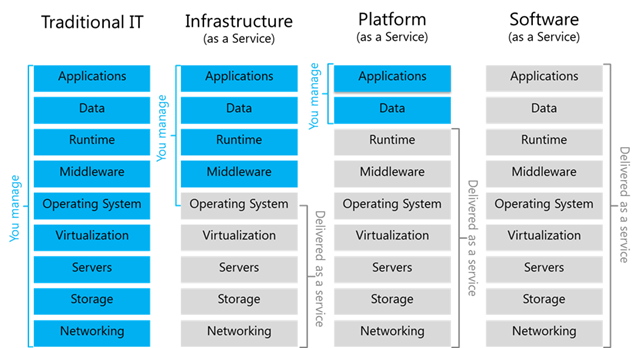
\includegraphics[width=1.0\textwidth]{fig/hauptteil/Service-Models.png}
  \caption{Die grundlegenden Cloud Service Modelle im Überblick}
  \centering
\end{figure}

\textbf{Infrastructure as a Service:} Der Nutzer hat die Fähigkeit Rechenleistung, Datenspeicher
Netzwerke und weitere fundamentale Computerresourcen bereitzustellen und beliebige Software
darauf zu betreiben, dazu können Betriebssysteme und Anwendungen gehören. Die
darunterliegende Infrastruktur wird vom Anbieter betrieben, der Nutzer  kann aber
eingeschränkte Kontrolle über bestimmte Komponenten haben, dazu gehören beispielsweise
Firewalls.

\textbf{Platform as a Service:} Der Nutzer verfügt über die Fähigkeit seine eingkaufte oder
selbst erstellten Anwendungen auf der Cloud Infrastruktur zu betreiben, die notwendige
Umgebung die über Sprachen, Bibliotheken, Tools und Services verfügt wird vom Anbieter
bereitgestellt. Die darunter liegende Infrastruktur mit Netzwerken, Servern,
Betriebssystemen und Speicher wird vom Anbieter betrieben, der Nutzer hat die Kontrolle
über die Anwendung und Konfiguration der Umgebung in der die Anwendung betrieben wird.

\textbf{Software as a Service:} Dem Nutzer wird der Zugriff auf die vom Anbieter in der
Cloud Infrastruktur betriebenen Softwareanwendung gewährt. Auf diese wird mithilfe
eines Thin oder Fat Clients zugegriffen, dabei kümmert sich der Nutzer nicht um den
Betrieb und die Konfiguration der darunterliegenden Cloud Infrastruktur wie
Netzwerke, Server, Betriebssystem, Speicher und die Anwendung selbst mit Ausnahme
eingeschränkter Nutzereinstellungen.

Die von NIST unterschiedenen grundlegenden Service Modellen können noch weiter
differenziert werden.
Ein Beispiel hierfür ist das Modell Function as a Service (FaaS) als Subset von PaaS.
FaaS erlaubt es Programmcode auszuführen ohne sich um die Bereitstellung weiterer 
Infrastruktur kümmern zu müssen wie es der Betrieb eines gewöhnlichen Microservices
verlangt.\\

In Art der Bereitstellung eines Cloud Services werden vier grundlegende Modelle
unterschieden; Public, Private, Hybrid und Community Cloud Modelle.\\

\textbf{Private Cloud:} Die Cloud Infrastruktur wird ausschließlich für die Nutzung durch eine einzige
Organisation mit mehreren Nutzern bereitgestellt. Besitz und Betrieb liegen dabei
entweder bei der selben Organisation, einer Drittpartei oder einer Kombination beider, 
die Infrastruktur kann dabei On- oder Off Premise betrieben werden.

\textbf{Public Cloud:} Die Public Cloud steht für die Nutzung durch die allgemeine Öffentlichkeit bereit.
Die Cloud Infrastruktur befindet sich im Besitz eines Unternehmens, Bildungseinrichtung,
Regierungsorganisation oder einer Kombination aus diesen und wird auch von der selben
Organisation On Premise betrieben. 

\textbf{Community Cloud:} Eine Community Cloud wird von einer Gemeinschaft von Nutzern mit gemeinsamen
Anliegen eingesetzt. Der Besitz und Betrieb liegen dabei bei einem oder mehreren
Mitgliedern dieser Gemeinschaft, einer Drittpartei und kann Off oder On Premise betrieben
werden.

\textbf{Hybrid Cloud:} Die Hybrid Cloud besteht aus einer Kombination der beschriebenen Modelle
(Public, Private und Community). Diese bilden dabei eigene Instanzen die aber durch
standardisierte oder proprietäre Schnittstellen den Transfer von Daten und Anwendungen
zwischen den Instanzen erlauben.

\subsection{Zu erwägende Vor- und Nachteile des Einsatzes von Cloud Computing}

\subsubsection{\textbf{Vorteile und Treiber der Adoption von Cloud Computing}}

\textbf{Wirtschaftliche Vorteile:} Ein Vorteil in der Nutzung von Cloud Computing
kann darin liegen dass ein Großteil der für den Betrieb notwendigen Infrastruktur
nicht mehr vom Unternehmen selbst eingakuft, eingerichtet und betrieben werden
muss (vgl. linke Seite Abb 2.1). Potentiell hohe Kosten die bereits vor der
Inbetriebnahme eines Systems mit einem höheren Risiko aufgewendet werden mussten
stellen in Form von individuell geringeren laufenden Beträgen ein deutlich
reduziertes Risiko da.\\
Sofern der Einsatz von Cloud Computing in einer sinnvollen und korrekten
Weise erfolgt können je nach Fall die Gesamtkosten um einen hohen Anteil reduziert
werden.\\
Die Gesamtkostenersparnisse stehen auch im Zusammenhang mit Skaleneffekten die für
große Cloudanbieter gelten. Der Betrieb eines einzelnen Servers ist im Verhältnis
mit bedeutend höheren Kosten verbunden als das hinzufügen eines äquivalenten
System zu einem Rechenzentrum im Betrieb von AWS oder einem vergleichbaren
Anbieter.

\textbf{Skalierbarkeit:} Besonders für schnell wachsende Unternehmen ist die
Option der schnellen Skalierbarkeit einer der prominentesten Vorteile der Cloud.
Es kann nicht nur auf vorhersagbare Anstiege (zum Beispiel ausgelöst durch
eine Verkaufsaktion) sondern auch auf unvorhersehbare Ereignisse reagiert werden.
Zusätzlich ist es möglich diese Skalierung nicht nur bis zu einem bestimmten Limit,
sondern nahezu unendlich zu betreiben. Wichtig ist auch dass sowohl auf steigende
als auch sinkende Nachfrage reagiert werden kann.

\textbf{Resilienz:} In einem worst case Szenario kann ein ganzes Rechenzentrum
durch unvorhergesehen Ereignisse wie beispielsweise Brände, Naturkatastrophen
oder anderes vollständig zerstört werden. Selbst wenn Backup-Rechenzentren
verfügbar sind ist eine übertragung der Operationen kein trivialer Ablauf und
birgt oft nicht außer Acht zu lassende Risiken. Die Flexibilität der Cloud
erlaubt es die gesamte Infrastruktur mit sehr geringem Aufwand in nicht
betroffene Regionen zu verlagern und die Kontinuität der Geschäftstätigkeiten
mit minimaler Unterbrechung aufrecht zu erhalten.

\textbf{Security:} Security Aspekte können sowohl einen Vor- als auch Nachteil
von Cloud Computings darstellen. Hier sollen zuerst Vorteile dargelegt werden,
potentielle Probleme werden im nächsten Unterkapitel beschrieben.
Die technischen Möglichkeiten und besonders auch die Wahrnung des Themas
Sicherheit in der Cloud unterlagen und unterliegen auch immernoch einem
deutlichen Wandel. Cloud Anbieter investieren
viele Resourcesn in Sicherheit und stellen dem Nutzer zum Beispiel bereits sicher
implementierte Verschlüsselungen zur Verfügung oder bieten einen gewissen
Schutzen vor Denial-of-Service Angriffen durch die natürliche Skalierbarkeit.\\

\subsubsection{\textbf{Nachteile und Risiken}}

\textbf{Netzwerkabhängigeit:} Da der Zugriff auf Cloud Dienste über das
Internet erfolgt entsteht dadurch entsprechend auch eine hohe Abhängigkeit.
Eine stabiele und schnelle Netzwerkanbindung ist vorraussetzung dass effektiv
gearbeitet werden kann, bei lokal gehosteten Systemen ist diese Abhängigkeit
entsprechend geringer.

\textbf{Vendor Lock-in:} Bei der Nutzung eines Cloud Anbieters entsteht die
Gefahr sich zu sehr in Abhängigkeit eines einzelenen Anbieters zu begeben.
Im Fall einer Änderung der Nutzungsbedingungen oder einer Änderung im
Bezahlmodell die den eignen Interessen stark entgegen steht besteht die Gefahr
bereits so abhängig von diesem Anbieter zu sein dass die Kosten eines Wechsels
derart hoch ausfallen dass man gezwungen ist die Bedingugen zu akzeptieren.

\textbf{Security und Privacy:} Sicherheitsrisiken sind einer der meistgenannten
Gründe die gegen Cloud Computing sprechen, besonders im Fall der Nutzung einer
Public Cloud. Die Gefahr dass Daten in die Hände dritter gelangen kann zum
zum Beispiel nicht vollständig ausgeschlossen werden. Da die Verantwortung über
die Sicherheit der Daten dem Cloud Anbieter unterliegt kann es auch zu Problemen
in Hinsicht der Privateheit der Daten kommen, sollte eine Regierungsorganisation
Zugriff auf bestimmte Daten eines Nutzer verlangen könnten diese ohne dessen
Einverständnis gewährt werden.

\textbf{Kosten:} Auch wenn die Nutzung von Cloud Computing mit dem Vorteil
geringerer Kosten beworben ist dies nicht zwingend garantiert. Werden die
vorhandenen Systeme ungünstig verwendet, zum Beispiel bleiben viele gebuchte
Ressourcen ungenutzt und IP-Adressen unverwendet, können hohe Kosten entstehen,
auch in der Phase des Übergangs zu Cloud Computing können höhere Kosten
entstehen als in einem vergleichbaren Zeitraum davor.


\subsection{Grundlegende Erklärung von DevOps}

Die exakte Definition und Abgrenzung des Begriffes DevOps ist ein Thema über
das es keine uniform akzeptierte allein gültige Definition und Abgrenzung gibt.
Im allgemeinen aber bezeichnet DevOps eine stärkere Vereinigung der Entwicklungs-
(Dev) und Betriebs- (Ops) Teams eines Softwareprojekts durch die Anwendung
einer effektiveren Arbeitskultur und -philosophie mit neuen Methoden, Werkzeugen und
Prozessen. Verschiedene Organisationen legen hierbei in ihrer Definition die
Schwerpunkte auf unterschiedliche Aspekte.
Als Beispiel betont Amazon hierbei besonders die schnelle Auslieferung neuer
Produkte ("ability to deliver applications and service at high velocity"),
Microsoft
die Kollaboration zwischen den beteiligten Teams ("DevOps enables formerly
siloed roles - development, IT operations, quality engineering, and security -
to coordinate and collaborate to produce better, more reliable products.").\\
Das DevOps Reasearch and Assessment (DORA) Team
hat über sieben Jahre mit 32.000 Beteiligten die Praktiken und 
Fähigkeiten untersucht die hohe Leistungsfähigkeit bei Entwicklung und
Auslieferung von Sofware fördern. Eine Übersicht über die Erkenntnisse dieser
Studie ist als Diagramm im Anhang ... zu finden.\\
Infrastructure as Code spielt als Werkzeug für die automatisierte Bereitstellung
der benötigten Computerresourcen eine wichtige Rolle im DevOps Prozess.

\subsubsection{\textbf{GitOps als Werkzeug für Continuous Devlivery im Rahmen von DevOps}}

GitOps wird von Gitlab als ein betriebliches Rahmenkonzept (operational
Framework) defniert das DevOps Best Practices in der automatiserten
Bereitstellung von Infrastruktur anwendet.
GitOps benötigt dabei drei Hauptkomponenten:\\
Infrastructure as Code, Merge Requests und CI/CD.
Organisationen die mit einer ausgereiften Anwendung der DevOps Kultur arbeiten
können über GitOps hunderte Male pro Tag neuen Code auf den Produktionsservern
installieren.

\subsection{Überblick über die wichtigsten Public Cloud Service Provider}
Da der Kern der Arbeit die Infrastructure as Code Unterstützung der
wichtigsten Cloud Service Provider in deren Public Cloud untersucht soll hier
ein kurzer Überblick über den aktuellen Markt in diesem Bereich gegeben werden.

\begin{figure}[H]
  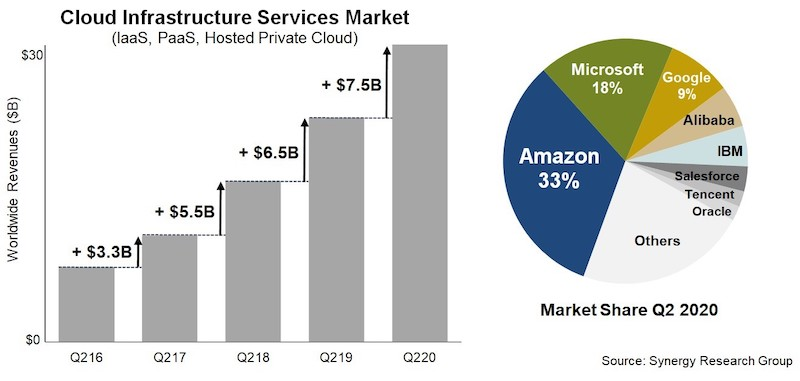
\includegraphics[width=1.0\textwidth]{fig/hauptteil/CIS_Q220.jpg}
  \caption{CSP Market Share Q2 2020 nach Umsatz}
  \centering
\end{figure}

\textbf{1. Amazon: } Amazon besitzt mit 33\% den größten Anteil am Markt.
Die Amazon Elastic Compute Cloud (EC2) ist die älteste der aktuell großen Cloud
Computing Plattformen, der erste Release fand im August 2006 statt.

\textbf{2. Microsoft: } Microsoft stellt den zweitgrößten Anteil am Markt mit
18\%, der erste Release von Microsoft Cloud Computing Service Microsoft Azure
erfolgte im Oktober 2008. Gemeinsam besaßen Amazon und Microsoft 2020 über 50\%
des gesamten Marktes.

\textbf{3. Google: } Google's Google Cloud Platform steht mit 9\% an dritter
Stelle. Google Compute Engine, die IaaS Komponente der Cloud Services von
Google wurde im Juni 2012 veröffentlicht.

\textbf{4. Alibaba Cloud: } Die viertgrößte Cloud Plattform ist die
Alibaba Cloud der Alibaba Group. Alibaba Cloud bietet zusätzlichzu seinem
Elastic Compute Service (ECS) einen dedizierte GPU basierten Service an. 

\textbf{5. IBM Cloud: } Die aktuell fünftgrößte Cloud Computing Plattform ist
die IBM Cloud von IBM. Bis Juni 2013 eine eigene Firma unter dem Namen Softlayer
wurde diese von IBM übernommen und 2017 gemeinsam mit den anderen Cloud Services
der Firma in ein einheitliches Portfolio unter dem Namen IBM Coud aufgenommen.\\

\begin{figure}[H]
  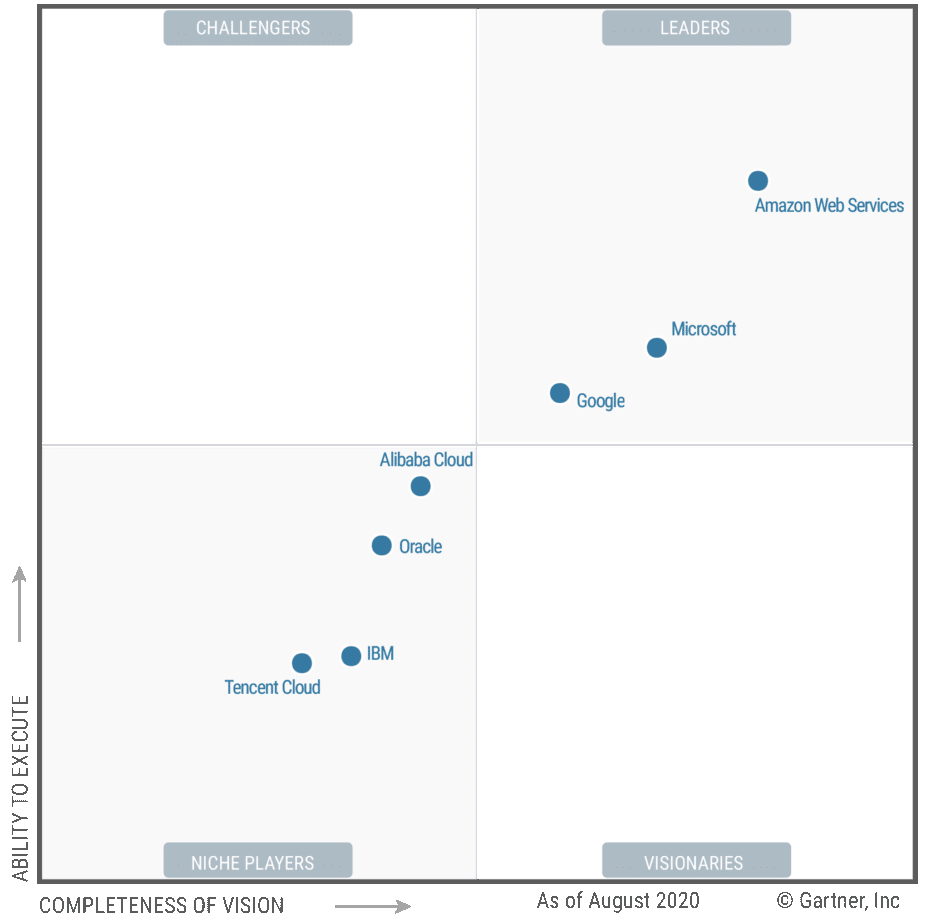
\includegraphics[width=1.0\textwidth]{fig/hauptteil/Gartner-Magic-Quadrant.png}
  \caption{CSP Gartner Magic Quadrant August 2020}
  \centering
\end{figure}

Der Gartner Magic Quadrant für Cloud Service Provider bietet einen groben
Überblick über den Umfang der Angebote (Completeness of Vision) und
die Ausgereiftheit einer Plattform (Ability to Execute). Deutlich erkennbar
ist hier die Vormachtsstellung von Amazon gegenüber Microsoft und Google sowie
der Abstand von Google zum nächst größten Anbieter Alibaba Cloud.
TODO: Irgendwas mit IBM Ability to Execute vs Marktanteil verglichen mit Oracle


\section{Was ist Infrastructure as Code?}

\subsection{Warum verwendet man IaC?}

\subsection{Technische Abgrenzung von IaC}

\section{Was ist Terraform?}

\subsection{Warum wird Terraform verwendet?}

\subsection{Terraform Alternativen und ergänzende Tools}

\section{Stand der Technik}

\chapter{Aufbau und Untersuchung}
\label{sec:real}
Beschreibung der HW- und SW-Realisierung

\section{High-level Aufbau der Infrastruktur des Versuchsobjekts}
\label{sec:real-unter}
Beispiel Text

\section{Zu analysiernde Aspekte und Eigenschaften}

\section{Konkreter Aufbau in Microsoft Azure}

\section{Konkreter Aufbau in Amazon AWS}

\section{Konkreter Aufbau in Google Cloud Platform}

\section{Literaturverweise}
\label{sec:real-literatur}

Verweise im Text: \cite{doc:stz} und \cite{doc:gun}.

\chapter{Ergebnisse}
\label{sec:ergeb}

\section{Bewertung Azure}

\section{Bewertung AWS}

\section{Bewertung GCP}

\section{Resultate und Vergleichsmatrix}

\enquote{Neuigkeiten} Messergebnisse
